\documentclass{article}
\usepackage{tikz}
\usepackage{amsmath}
\usetikzlibrary{angles,quotes}
\begin{document}
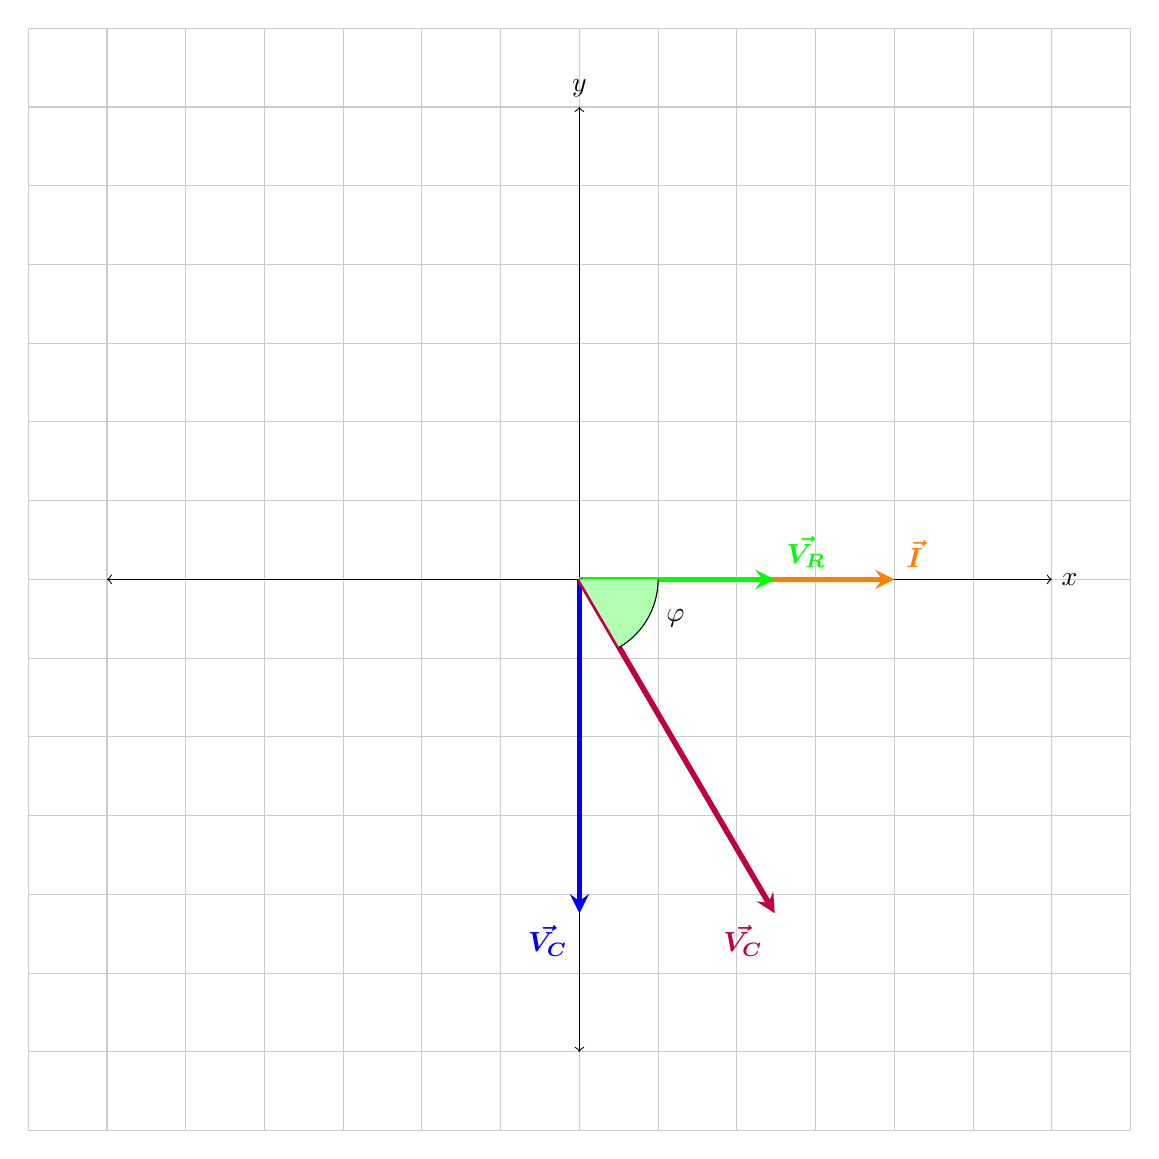
\begin{tikzpicture}
  \draw[thin,gray!40] (-7,-7) grid (7,7);
  \draw[<->] (-6,0)--(6,0) node[right]{$x$};
  \draw[<->] (0,-6)--(0,6) node[above]{$y$};
  \draw[line width=2pt,orange,-stealth](0,0)--(4,0) node[anchor=south west]{$\boldsymbol{\vec{I}}$};
  \draw[line width=2pt,green,-stealth](0,0)--(2.48,0) node[anchor=south west]{$\boldsymbol{\vec{V_R}}$};
  \draw[line width=2pt,blue,-stealth](0,0)--(0,-4.24) node[anchor=north east]{$\boldsymbol{\vec{V_C}}$};
  \draw[line width=2pt,purple,-stealth](0,0)--(2.48,-4.24) node[anchor=north east]{$\boldsymbol{\vec{V_C}}$};
%angolo

%\draw [fill=green!30] (a) -- ++(1cm,0) arc(0:{atan(1/2)}:1cm) node[midway,right] {$\alpha$} -- cycle;
\coordinate (a) at (0,0);
\coordinate (b) at (2.48,0);
\coordinate (c) at (2.48,-4.24);


\draw pic[draw,fill=green!30,angle radius=1cm,"$\varphi$" shift={(7mm,-2mm)}] {angle=c--a--b};



\end{tikzpicture}
\end{document}
